\documentclass{article}
\PassOptionsToPackage{hyphens}{url}
\usepackage[hidelinks]{hyperref}
\usepackage{amsmath}
\usepackage{amsthm}
\usepackage{amssymb}
\usepackage{pgfplots}
\usepackage{algpseudocode}
\newcommand{\QED}{\hfill {\qed}}
\newcommand\tab[1][1cm]{\hspace*{#1}}
\usepackage{mathtools}
\DeclarePairedDelimiter\ceil{\lceil}{\rceil}
\DeclarePairedDelimiter\floor{\lfloor}{\rfloor}
\graphicspath{ {./imgs/} }

\title{\#3 Assignment - CMPT 405}
\author{Luiz Fernando Peres de Oliveira - 301288301 - lperesde@sfu.ca}

\begin{document}

\maketitle
\textbf{\#1a)}
\\
Let $G_1$ be a graph with two vertices $A$ and $B$ and an edge $(A, B)$ with weight $1$. For every shortest path tree $T_v$, $v \in V$, $T_v$ is also a MST (it is easy to see, as there is only one tree).
\\
\\
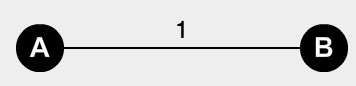
\includegraphics[scale=0.6]{simple_graph_hw3}
\\
\\
\textbf{\#1b)}
\\
Let $G_2$ be a graph with vertices $A, B, C$ and $D$ and edges $(A, B), (A, D), (A,C), (B,C)$ and $(C,D)$, with weights $8, 4, 6, 4 \text{ and } 8$, respectively. Then, no shortest path tree $T_v$ given by Dijkstra's algorithm is a MST.
\\
\\
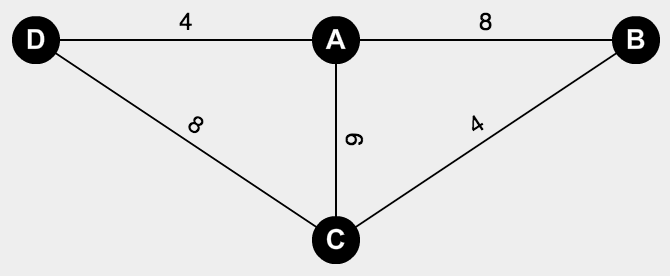
\includegraphics[scale=0.4]{complex_graph_hw3}
\\
\\
MST $= (A,C), (A,D), (B,C)$
\\
$T_a = (A, B), (A, C), (A, D)$
\\
$T_b = (A, B), (A, D), (B, C)$
\\
$T_c = (A, C), (B, C), (C, D)$
\\
$T_d = (A, B), (A, D), (C, D)$
\\
\\
\textbf{\#2)}
\\
\textbf{\#3)}
\\
The idea of the algorithm is to use an approach similar to the Floyd-Warshall algorithm for transitive closures, as transitive reductions are essentially the inverse of transitive closures. In Floyd-Warshall, we augment the number of edges whenever we find a path $i \rightarrow k \rightarrow j$ with total weight less than the weight of the path $i \rightarrow j$. However, in transitive reduction, we are interested in minimizing the number of edges that are used, thus, we always prefer paths $i \rightarrow j$ than $i \rightarrow k \rightarrow j$. The algorithm is very straightforward and can be thought as a modification of Floyd-Warshall and has same complexity ($O(n^3)$):
\\
Algorithm:\\
\textbf{Input:} $G=(V,E)$
\begin{algorithmic}
\State $E' \gets$ copy $E$
\For{$i$ \textbf{from} $1$ to $n$}
  \For{$j$ \textbf{from} $1$ to $n$}
    \For{$k$ \textbf{from} $1$ to $n$}
      \If{$\{(i, j), (i, k), (k, j) \} \subseteq E'$, where $(i,j) \neq (i, k) \neq (k, j)$}
        \State $E' \gets E' - (i, k)$
      \EndIf
    \EndFor
  \EndFor
\EndFor
\State \textbf{return} $G'=(V, E')$
\\
\end{algorithmic} 
\textbf{\#4)}
\\
Let $T$ be the unrooted tree decomposition of $G$ and $T'$ be a nice tree decomposition of $T$. The idea of the algorithm is to make any node of $T$ (preferably a internal node with many edges or minimum bag width) its root. So to ease the algorithm, we  preprocess the input $T$: after we root $T$, we go through all the bag leaves $b$ in $T$ and create a new bag for every $v_b \in (b - parent(b))$ and make $b$ their parent. We then run a postorder traversal on $T$ and apply the following rules:
\\
- \textbf{Case 1.} If bag $b$ is a leaf in $T$:
\\
\tab If $b \neq parent(b)$, it must have come from the preprocessing of the original bag $b' - parent(b')$, and therefore $|b| = 1 \leq |parent(b)|$, meaning that we need to add introduce nodes to our nice tree decomposition $T'$ by adding some vertices $v_{parent} \in parent(b)$ and stop when they have the same elements, so we can join the bags later; otherwise, if $b$ and $parent(b)$ have the same elements, we are done.
\\
\\
- \textbf{Case 2.} If bag $b$ is an internal node in $T$:
\\
\tab We know that if $b$ is an internal node, then $b$ is a parent of at least one bag $b'$.  Then, the first step is to add a join node in $T'$ for $b$ and every $b'$, where $parent(b') = b$. Also, because $b$ is an internal node, $b$ has a parent. We need first to get rid of all nodes in $b$ that are not elements of $parent(b)$ (by adding forget nodes to $T'$) and finally add some vertices  $v_{parent} \in parent(b)$ and stop when $b$ and $parent(b)$ have the same elements, so we can join the bags later (by adding introduce nodes to $T'$).
\\
\\
- \textbf{Case 3.} If bag $b$ is the root in $T$:
\\
\tab Finally, if $b$ is the root, we only need to create a join node of all bags $children(b)$ in our final nice tree decomposition $T'$.
\\
\\
The algorithm runs in $O(nk)$ (as per the pseudocode and demonstration below)
\\
\\
Algorithm:\\
\textbf{Input:} \textit{T}
\begin{algorithmic}
\State Make any internal bag (or the bag with minimum width) of $T$ its root.
\For{\textbf{each} bag $b \in T, children(b) = \emptyset $} \textit{// all leaves}
  \State $free_{vs} \gets b - parent(b)$
  \For{\textbf{each} $v \in free_{vs}$}
    \State $T \gets T \cup \{v \}$ such that $parent(v) = b$
  \EndFor
\EndFor
\State $T' \gets \emptyset $
\For{\textbf{each} bag $b \in T_{postorder}$}
  \State $b_{aux} \gets b$
  \If{$children(b) = \emptyset$} \textit{// if leaf}
    \State $T' \gets T' \cup b_{aux}$ \textit{// add leaf node}
    \While{$b_{aux} \neq parent(b)$ }
      \State add introduce node $b_{aux} \cup \{ v_{parent}\} $ in $T'$, for any $ v_{parent} \in parent(b)$,
      \State such that $b_{aux} \cup \{ v_{parent}\} = parent(b_{aux})$
    \EndWhile
  \Else
    \State Create join node in $T'$
    \If{$parent(b) \neq \emptyset$} \textit{// if not root}
      \While{$\exists v \in b \text{, such that } v \notin parent(b)$}
      \State add forget node $b_{aux} - \{ v\} $ in $T'$, for any $ v \notin parent(b)$,
      \State such that $b_{aux} - \{ v\} = parent(b_{aux})$
      \EndWhile
      \While{$b_{aux} \neq parent(b)$ }
      \State add introduce node $b_{aux} \cup \{ v_{parent}\} $ in $T'$,
      \State for any $ v_{parent} \in parent(b)$, such that $b_{aux} \cup \{ v_{parent}\} = parent(b_{aux})$
    \EndWhile
    \EndIf
  \EndIf
\State
\EndFor
\State \textbf{return} $T'$
\end{algorithmic} 
\newpage
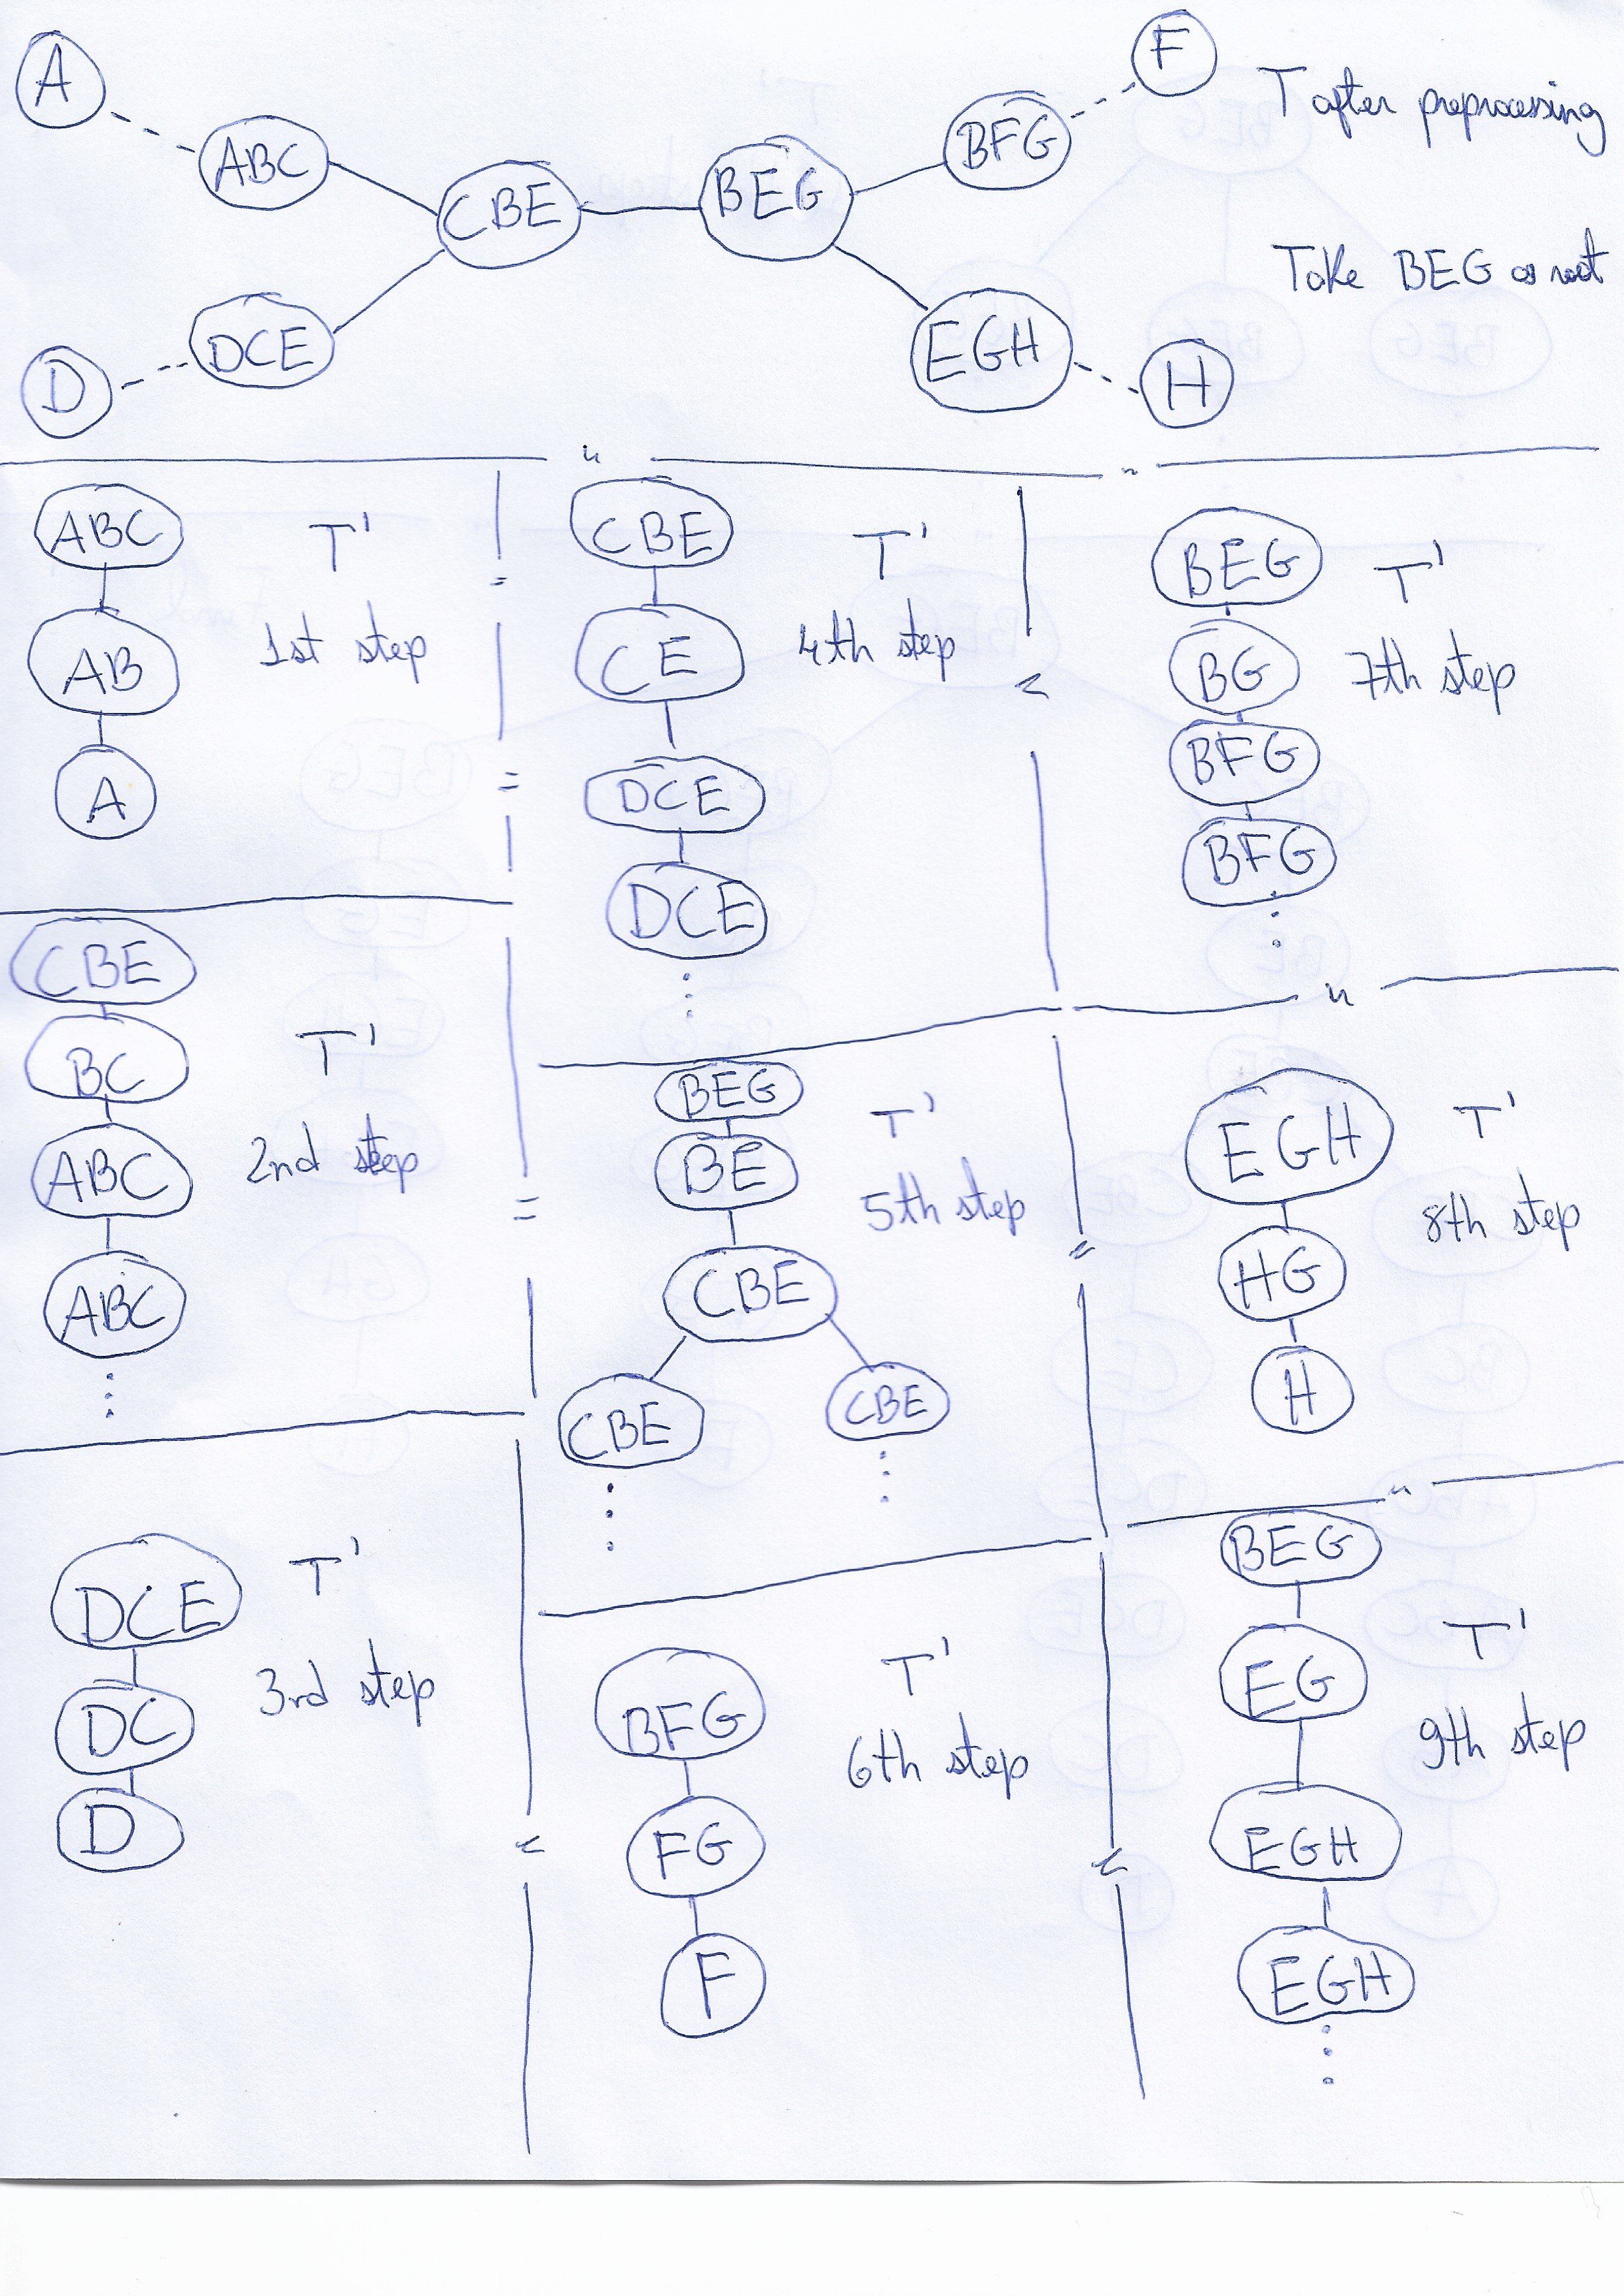
\includegraphics[scale=0.7]{1st_demo_graph_hw3}
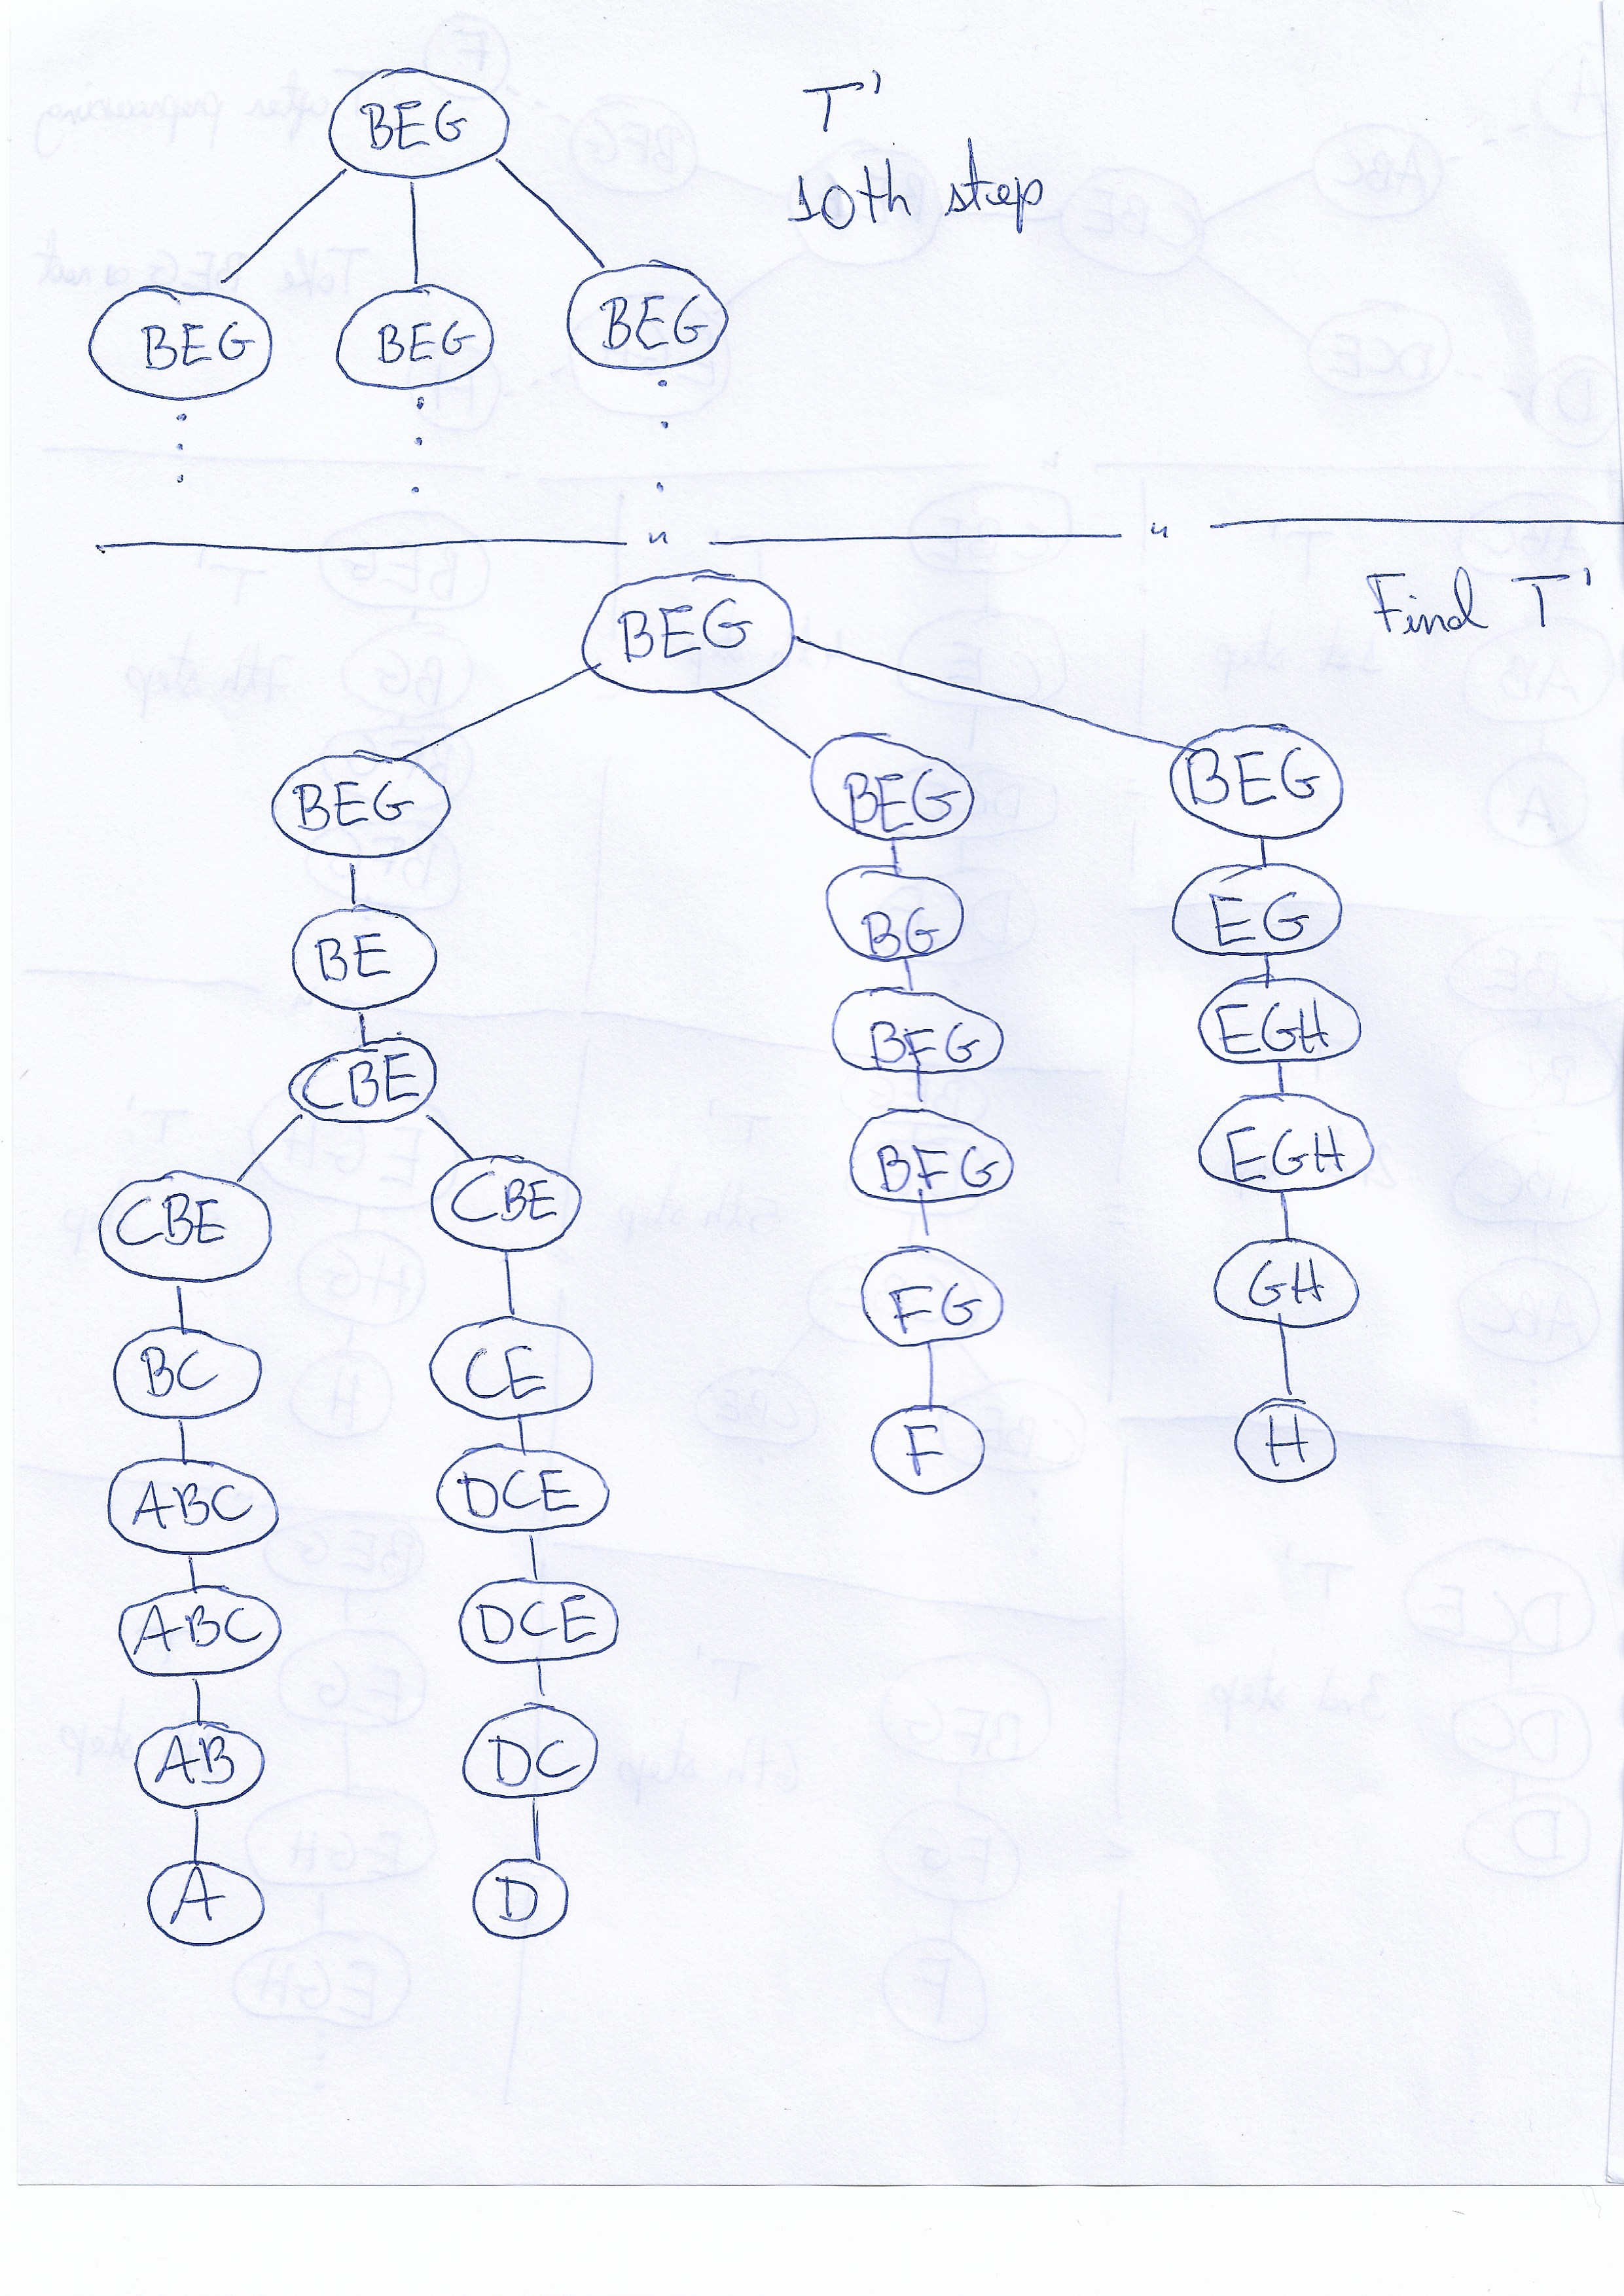
\includegraphics[scale=0.7]{2nd_demo_graph_hw3}
\\
\\
\textbf{Note.:} I know joins are only possible with two bags. It was too late to fix that when I realized I did this mistake in my examples and algorithm on \#4, please ignore it. Imagine we made $T$ a binary tree and worked from there (check image on question \#5).
\\
\\
\textbf{\#5)}
\\
\textit{Definition:} (As per lecture 17). Let $B_x$ be the vertices appearing in node $x$ and let $V_x$ be the vertices in the subtree rooted at $x$. Let $M[x, S]$ be a matrix that keeps the size a maximum independent set $I \subseteq V_x$ with $I \cap B_x = S$. At the end of the algorithm, the maximum independent set size will them be on $M[root, S'_{root}]$, where $S'_{root}$ is the best $S$ for the root.\\
\\
\textit{Recurrence:}
\\
\\
\textbf{- Leaf:} $B_x$ has no children
\\
$M[x, S] = 1$
\\
\\
\textbf{- Introduce:} 1 child $y$, $B_x = B_y \cup \{v\}$, for some vertex $v$
\begin{gather*}
M[x, S] =
\begin{cases}
M[y, S] \tab\tab\text{ if $v \notin S$ } \\
M[y, S - \{v\}] + |v| \tab\text{if $v \in S$ but $v$ has no neighbor in $S$ }\\
-\infty \tab\tab\text{   }\text{ if $S$ contains $v$ and its neighbors }
\end{cases}
\end{gather*}\\
\\
\textbf{- Forget:} 1 child $y$, $B_x = B_y - \{v\}$, for some vertex $v$
\\
$M[x, S] = max\big(M[y, S], M[y, S \cup \{v\}]\big)$
\\
\\
\textbf{- Join:} 2 children $y_1, y_2$, $B_x = B_{y1} = B_{y2}$
\\
$M[x, S] = M[y_1, S] + M[y_2, S] - |S|$
\\
\\
Algorithm:\\
\textbf{Input:} $T', root$
\begin{algorithmic}
\For{\textbf{each} $x \in T'{postorder}$}
  \For{\textbf{each} $I \subseteq V_x$ with $S = I \cap B_x$}
    \State compute recurrence $M[x, S]$ as described above
    \State keep best $S$ in $S'$ for every $x$
  \EndFor
\EndFor
\State \textbf{return} $M[root, S'_{root}]$\\
\end{algorithmic}
\textit{Demonstration:}
There are at most $2^{k+1}\times n$ subproblems (entries) in $M$ and therefore its running time is bounded on $M$. Demonstrate that would take a matrix of size $2^4 \times 25$, which is very large. Thus, the image below summarizes it:
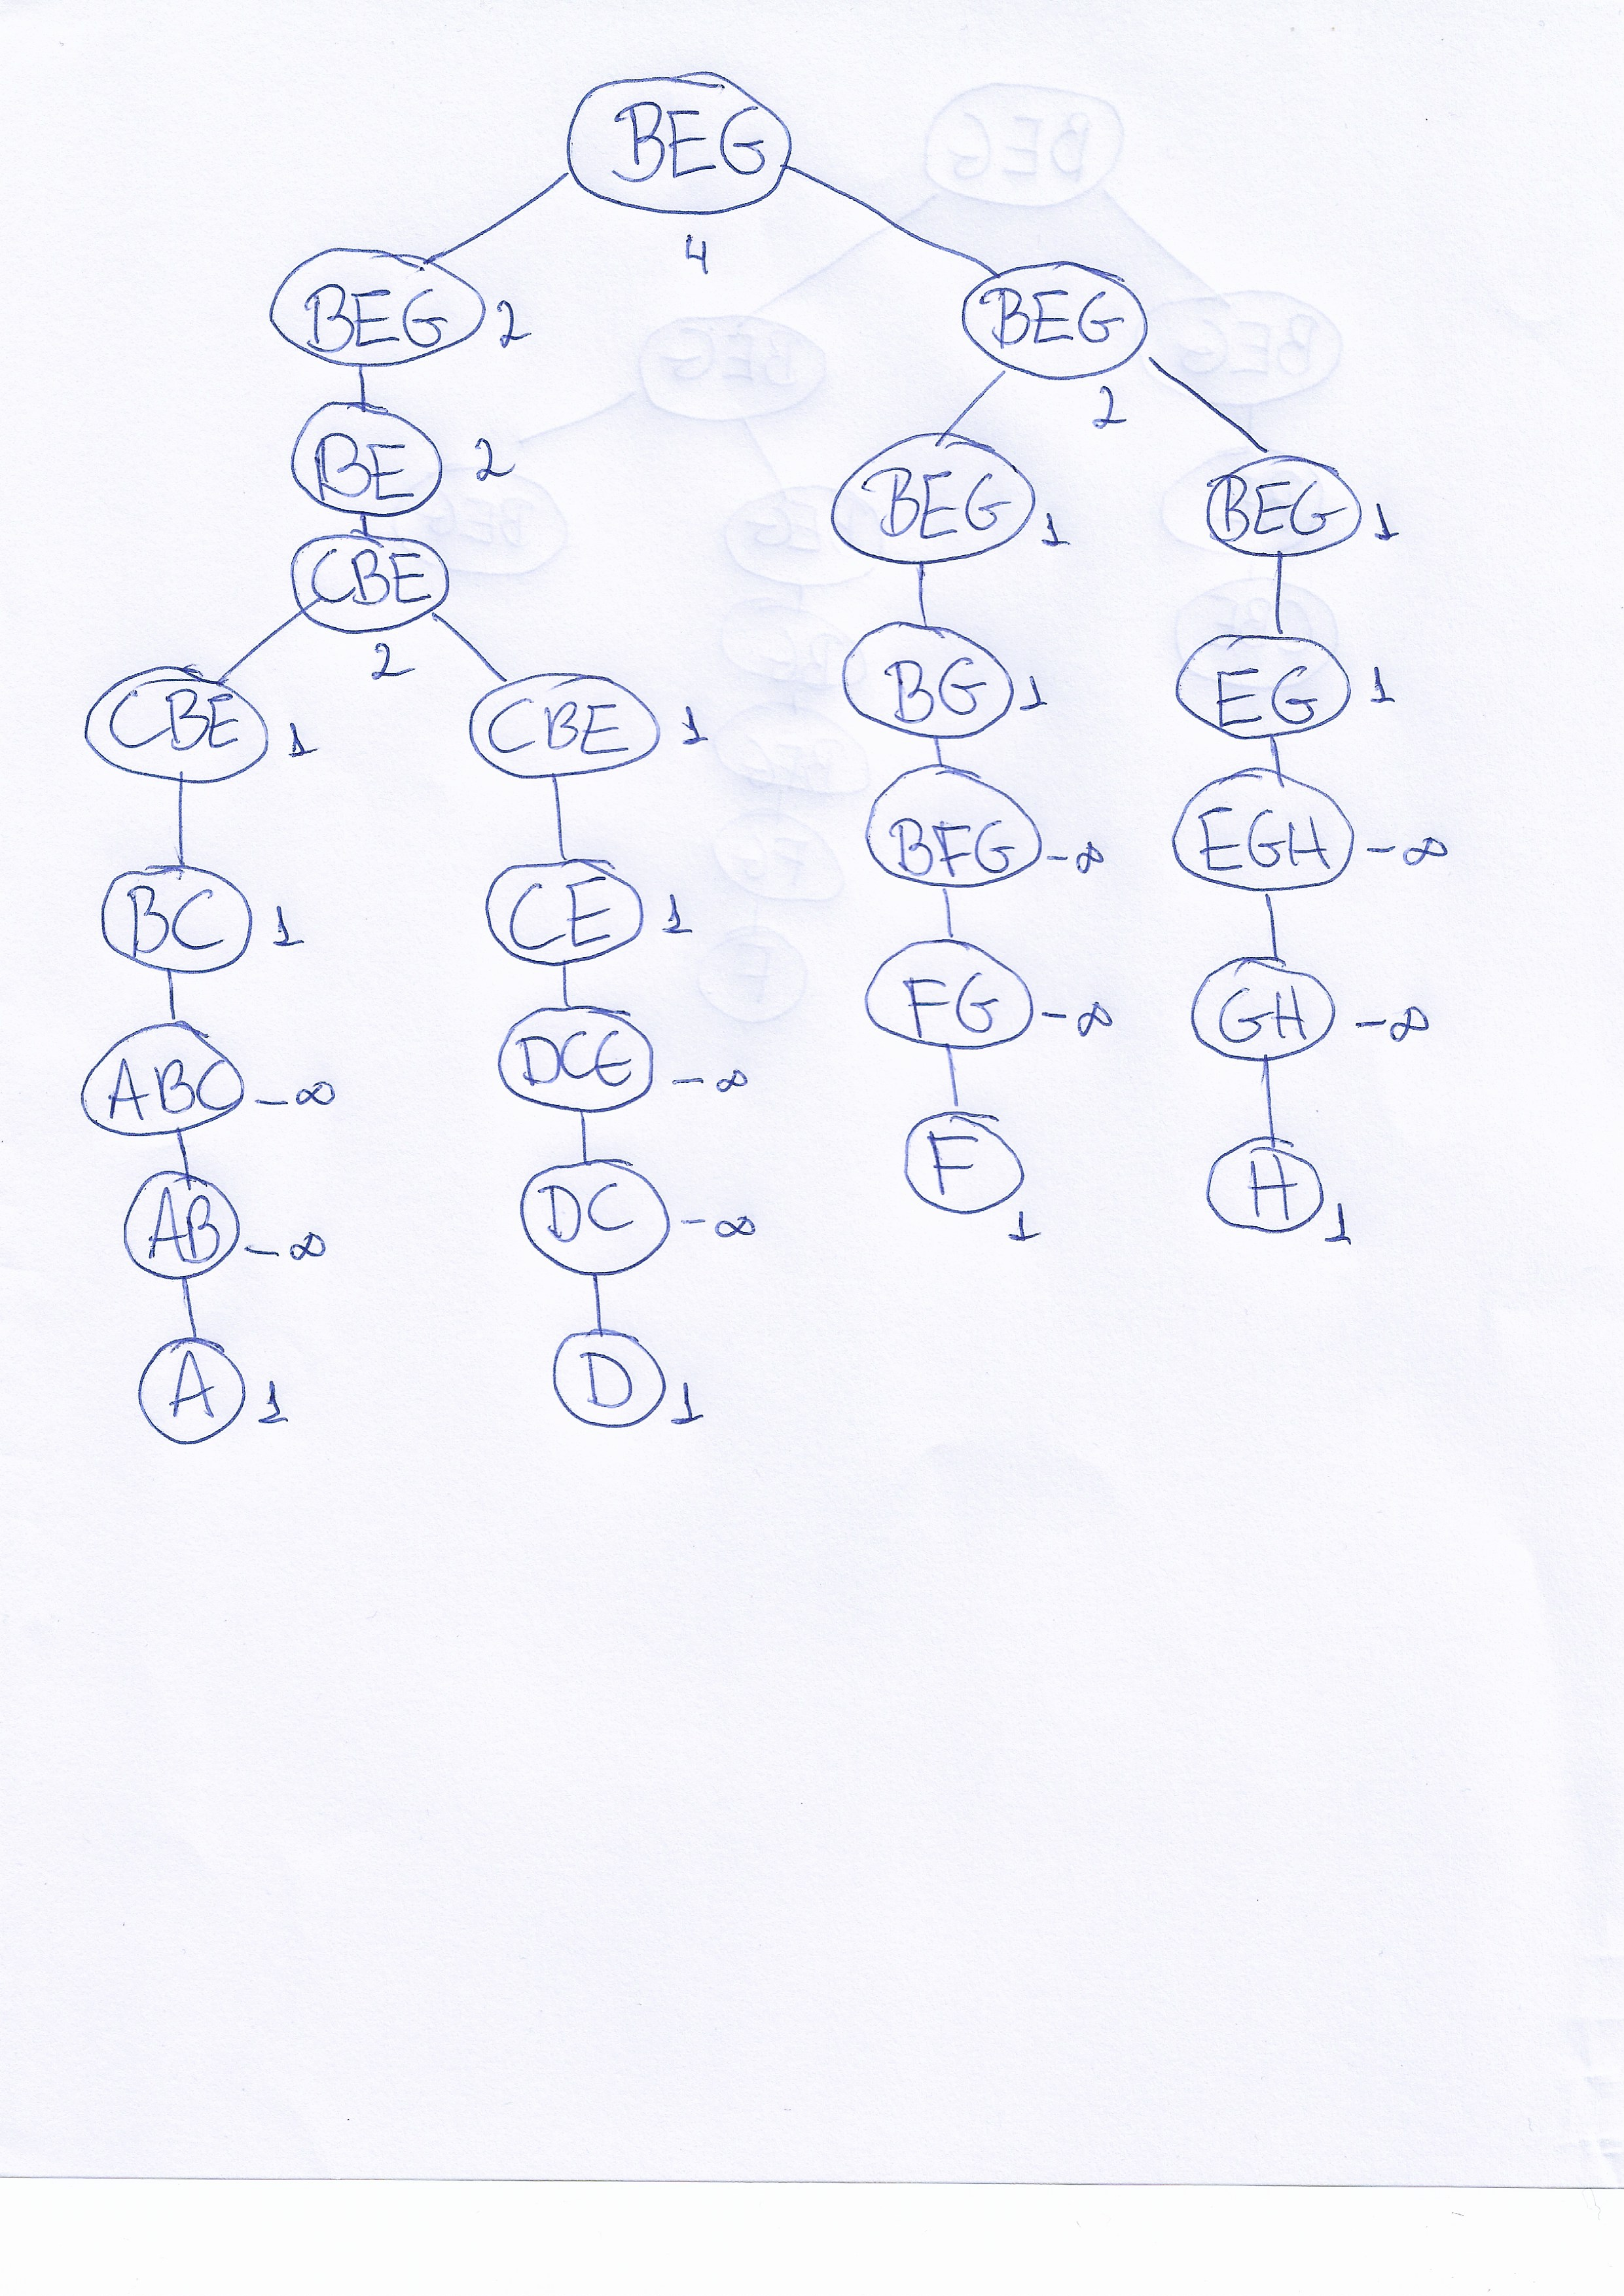
\includegraphics[scale=0.7]{3rd_demo_graph_hw3}
\end{document}